\documentclass[swedish,a4paper,onepage, 11pt]{scrbook}

\usepackage[T1]{fontenc}
\usepackage[utf8]{inputenc}
\usepackage{babel}
\pagestyle{headings}
\setcounter{tocdepth}{3}
\setlength\parskip{\medskipamount}
\setlength\parindent{0pt}
\setlength{\unitlength}{1cm}
\addtolength{\textheight}{2cm}
\usepackage{multicol}

\usepackage{graphicx}
\usepackage{ae}
\usepackage{aecompl}
\usepackage{amssymb}
\usepackage{amsmath}
%\usepackage{bookman}
\usepackage{multicol}
\usepackage{gensymb}
\usepackage{listings}
\usepackage{pdfpages}




\usepackage{geometry}
%\areaset[-2cm]{18cm}{26cm}

%\linespread{0.9}


\begin{document}

\newcommand{\tavla}[1]{\reversemarginpar{ \rule[-10mm]{0.1mm}{#1cm}}}
\newcommand{\svarsrad}{\begin{flushright} \rule{7cm}{0.2mm} \end{flushright}}
\newcommand{\asm}[1]{\texttt{\textbf{#1}}}

\newcommand{\startex}[1]{\textbf{Example}\begin{quote}#1\end{quote}}
\newcommand{\slutex}{\begin{flushright}\rule{1ex}{1ex}\end{flushright}}


\title{Sun's position for navigation with DM15L\\{}Manual\\{}}

\author{Michael Josefsson}
\date{\today}
\maketitle

\addtolength{\evensidemargin}{-2.0cm}
\addtolength{\oddsidemargin}{2.0cm}

\subsection*{Overview}

The handheld calculator DM15 (a HP-15c look-a-like with more memory) can be used for determining the sun's position with precision enough for celestial navigation purposes. The accompanying program, listed in the Appendix, constitutes a handy tool for either finding the \emph{Nautical Almanac}'s entries GHA (\emph{Greenwich Hour Angle}) and Declination, or --- with AP (\emph{Assumed Position}) --- directly calculate the sun's Altitude \emph{Hc} and Azimuth \emph{Az} for this position.

The algorithm relies on pure Keplerian motion of the sun. No planetary perturbations are taken into account. Resulting angular accuracy is about 1 minute of arc, which is adequate for general navigation at sea.

\chapter{Usage} 

Before use, notice that: 

\begin{itemize}
\item All times entered are UT (''GMT'') even if observer's longitude is not the prime meridian. Of course, local hour angles take longitude into consideration, but all times are still UT. Time format is $hh.mmss$, where $mm$ and $ss$ must be two-digit numbers.


\item The program makes use of the calculator's internal decimal to degrees, minutes and seconds routines both for \textbf{entry} and \textbf{displayed result}. In navigation a more common format of degrees, minutes and tenths of a minute is used. That conversion, if needed, is readily done by dividing the arc-seconds number or multiplying the minute's decimal by 6.

\startex{Convert angle in $ddd.mmss$ to $ddd.mm{\cdot}t$}

 $98\degree\, 26'\, 12''$, entered as \asm{98.2612},  is $98\degree\, 26{\cdot}2'$ where $12''/6=2$\\
 $98\degree\, 26'\, 43''$, entered as \asm{98.2643}, is $98\degree\, 26{\cdot}7'$ where $43''/6\approx7$
 \slutex
 
\startex{Convert angle in $ddd.mm{\cdot}t$ to $ddd.mmss$}

 $14\degree\, 7{\cdot}3'$  is $14\degree\, 7'\, 18''$ where $3 \cdot 6=18$\\
 $277\degree\, 4{\cdot}5'$  is $277\degree\, 4{\cdot}30'$ where $5 \cdot 6=30$
 \slutex
 
\end{itemize}
 
\section{User-defined  buttons} 

The programs user-defined functions are accessed via the buttons below

\begin{center}
\begin{tabular}{ll}
Button & Function \\
\hline
\textbf{\textsf{A}} & Date for Aries angle at UT=0h\\
\textbf{\textsf{B}} & Time for Sun Altitude and Azimuth \\
\textbf{\textsf{C}} & SHA and declination for \emph{own object} \\
\textbf{\textsf{D}} & Time for \emph{own object}'s Altitude and Azimuth \\
\textbf{\textsf{E}} & Time for GHA Aries and LHA Aries\\
\textbf{\textsf{.5}} & After \textbf{\textsf{B}} for GHA and declination\\
& (as a Nautical Almanac entry)\\
\end{tabular}
\end{center}

\section{Assumed Position} An AP (\emph{Assumed Position}) is entered in registers \asm{\textbf{8}} and \asm{\textbf{.8}} before any calculations can be peformed.

\startex{Entering AP.} A location of Lat N$58\degree\, 34'$, Long E$14\degree\, 34'\,12''$ is entered into registers \asm{\textbf{8}} and \asm{\textbf{.8}}:

\begin{center}
\begin{tabular}{c|c|l|l|l}
Data       & Format      & Key  &Display shows&Meaning\\
\hline
\asm{58.3400} & $\pm dd.mmss$ & g$\rightarrow$H \asm{STO 8} &\asm{58.5667} & Decimal degrees\\
\asm{14.3412} & $\pm dd.mmss$ & g$\rightarrow$H \asm{STO .8} &\asm{14.5700}& Decimal degrees\\
\end{tabular}
\end{center}

East and North are positive, West and South are negative. \\The position is permanently stored until manually changed and need only be set once.
\slutex

\section{Daily entry} Every day has its own parameters that require the \asm{\textbf{A}}-routine to be run once for each day.

\startex{Entering the date.} Enter June 12th 2022, i.e. year 2022, month 6 and day 12.

\begin{center}
\begin{tabular}{c|c|r|l|l}
Data       & Format      & Key  &Display shows&Meaning\\
\hline
\asm{2022} &  $YYYY$   & ENTER &\asm{2022.0000}\\
\asm{6} &  $mm$   & ENTER &\asm{6.0000}\\
\asm{12} &  $dd$   & f \asm{\textbf{A}} &\asm{260.1816}& $260\degree\, 18'\,16''$, GHA Aries at 0h\\
&&&&(\emph{Nautical Almanac 2022}:  $260\degree\,18'{\cdot}1$)\\ 
\end{tabular}
\end{center}

\slutex 

\section{Sun's Altitude and Azimuth} Next the sun's position for time of date UT/GMT can be  calculated.

\startex{Find sun's Hc and Az for UT 09h 54m 48s. Date as above.} Enter time in format $hh.mmss$ then use routine \asm{\textbf{B}}.

\begin{center}
\begin{tabular}{c|c|r|l|l}
Data       & Format      & Key  &Display shows&Meaning\\
\hline\asm{9.5448} &  $hh.mmss$   & f \asm{\textbf{B}} &\asm{52.3845} & Hc = $52\degree\, 38'\,45''$ \\
&    &  \asm{\textbf{x<>y}} &\asm{154.1140} & Az = $154\degree\, 11'\,40''$ \\
\end{tabular}
\end{center}

\textbf{Result:} Hc = $52\degree\, 38{\cdot}7'$, Az = $154\degree$

A new time can be entered directly. For example, also find sun's Hc and Az a few minutes later at UT 10h 02m 30s. 

\begin{center}
\begin{tabular}{c|c|r|l|l}
Data       & Format      & Key  &Display shows&Meaning\\
\hline
\asm{10.0230} &  $hh.mmss$   & f \asm{\textbf{B}} &\asm{53.0338}&  Hc = $53\degree\, 03'\,38''$ \\
&    &  \asm{\textbf{x<>y}} &\asm{157.0236}&  Az = $157\degree\, 2'\,36''$ \\
\end{tabular}
\end{center}

\textbf{Result:} Hc = $53\degree\, 03{\cdot}6'$, Az = $157\degree$

\slutex

\section{GHA and declination} 
The program can also produce values for GHA and declination imitating the \emph{Nautical Almanac}.

\startex{Find GHA and decl for 10h on June 12th 2023} After calculating Hc and Az as above, use \asm{\textbf{GSB .5}} to get GHA and declination $\delta$:

\begin{center}
\begin{tabular}{c|c|r|l|l}
Data       & Format      & Key  &Display shows&Meaning\\
\hline
\asm{10.0000} &  $hh.mmss$   & f \asm{\textbf{B}} &\asm{52.5508} &Hc = $52\degree\, 55'\,08''$\\
&    &  \asm{\textbf{GSB .5}} &\asm{330.0248} & GHA = $330\degree\, 2'\,48''$ \\
&    &  \asm{\textbf{x<>y}} &\asm{23.0901} & $\delta$ = $23\degree\, 09'\,01''$ \\
\end{tabular}
\end{center}

\textbf{Result:} GHA = $330\degree\, 2{\cdot}8'$, Decl = $23\degree\, 09{\cdot}0'$ (\emph{Nautical Almanac} gives $330\degree\, 2{\cdot}8'$ and $23\degree\, 8{\cdot}8'$).

GHA and Decl can of course be calculated for any other time during the day in the same manner. 
\slutex

\section*{Specify and calculate position for an object with known SHA and declination} 

The coordinates of a celestial object, for example a star, are given as SHA (\emph{Sidereal Hour Angle}) and declination.\footnote{Right Ascension can be entered as $\alpha=360 - SHA$ if needed.}

\startex{Enter coordinates of \emph{Vega} (SHA $80\degree\, 34{\cdot}3'$, declination $38\degree\, 48{\cdot}2'$).}

\begin{center}
\begin{tabular}{c|c|r|l|l}
Data       & Format      & Key  &Display shows&Meaning\\
\hline
\asm{80.3418} &  $ddd.mmss$   & ENTER &\asm{80.3418}&SHA\\
\asm{38.4812} &  $ddd.mmss$   & f \asm{\textbf{C}} & \asm{279.4283}& RA in decimal degrees\\
\end{tabular}
\end{center}


Now find \emph{Vega}'s calculated position for UT = 23h 02m 10s on June 12th 2023 already entered above.

\begin{center}
\begin{tabular}{c|c|r|l|l}
Data       & Format      & Key  &Display shows&Meaning\\
\hline
\asm{23.0210} &  $hh.mmss$   & f \asm{\textbf{D}} &\asm{67.0015} & Hc = $67\degree\, 00'\,15''$  \\
&    &  \asm{\textbf{x<>y}} &\asm{141.1224} & Az = $141\degree\, 12'\,24''$ \\
\end{tabular}
\end{center}

\textbf{Result:} Vega can be expected at \emph{Hc} = $67\degree\, 0{\cdot}2'$ and \emph{Zn} =  $141\degree$. Set the sextant for $67\degree$ and search for it in south-east.
\slutex

\section*{GHA Aries and LHA Aries} 

Find GHA Aries on 4 October 2022 at 7h 57m 20s. Also find LHA Aries longitude in \asm{.8} ($14\degree\, 34'\,12''$ E as before).

\begin{center}
\begin{tabular}{c|c|r|l|l}
Data       & Format      & Key  &Display shows&Meaning\\
\hline
\asm{2022} &  $YYYY$   & ENTER &\asm{2022.0000}& Year\\
\asm{10} &  $mm$   & ENTER &\asm{10.0000} & Month\\
\asm{4} &  $dd$   & f \asm{\textbf{A}} &\asm{12.4006} &$12\degree\, 40'\,6''$, GHA Aries at 0h\\
\asm{7.5720} &  $hh.mmss$   & f \asm{\textbf{E}} &\asm{132.1942} & GHA Aries = $132\degree\, 19'\,42''$ \\
&    &  \asm{\textbf{x$\leftrightarrow$y}} &\asm{146.5354} & LHA Aries = $146\degree\, 53'\,54''$ \\
\end{tabular}
\end{center}

\section*{Use as \emph{Sight Reduction Table}} 

The program can also solve the navigational triangle and be used as a  \emph{Sight Reduction Table} replacement (Ho-214/Ho-229~etc). To solve the triangle  1) AP latitude, 2) object's declination and 3) hour angle need to be entered.

AP latitude is entered in register \asm{8} as before, declination is set via \textbf{\textsf{C}} and hour angle is entered into register \asm{.2}. The hour angle is positive if westward.

\startex{Find Hc and Az as in Ho-214} Assume latitude N$58\degree$, Declination $8\degree\, 30'$ and an hour angle of $54\degree$ (object to the west of observer).

\begin{center}
\begin{tabular}{c|c|r|l|l}
Data       & Format      & Key  &Display shows&Meaning\\
\hline
\asm{58} &  $dd.mmss$   & \asm{STO 8} &\asm{58.0000}& Decimal latitude \\
\asm{8.3000} &  $dd.mmss$   & \textbf{\textsf{C}} &\asm{8.5000}& Decimal declination\\
\asm{54}     &  $dd.mmss$   & g$\rightarrow$H & \asm{54.0000} & Decimal Hour angle\\
             &              & \asm{STO .2} & \asm{54.0000}\\
             &              & \asm{GSB 7} & \asm{25.4102} & Hc = $25\degree\, 41'\,02''$\\
             &              &  \asm{\textbf{x$\leftrightarrow$y}} &\asm{242.3616} & Az = $242\degree\, 36'\,16''$ = 242.6\degree\\
\end{tabular}
\end{center}

Ho-214 gives Alt. = $25\degree\, 41{\cdot}0'$ and  Az. = $117.4\degree$. Where true azimuth is $360-117.4=242.6\degree$. 


\appendix

\chapter{Program and information}
\subsection*{Register usage}
The lower registers \asm{r0..r7} are used by the calculator's statistics functions and are not \emph{permanently} used by this program. They \emph{are} used however for intermediate results via the normal operating sequences \textbf{\textsf{A-B}} or \textbf{\textsf{A-C-D}} or \textbf{\textsf{A-E}}.

In short: Use \asm{r0..r7} as you wish but they will be altered by \textbf{\textsf{A}}.

\subsection*{Program installation}

For a fresh install of the program perform steps 1--6 below.

\begin{enumerate}

\item Make space on the DM15 for program and registers:
\begin{itemize}
 \item Enter \asm{\textbf{21 f DIM (i)}}  
 
 \item Double check:  \asm{\textbf{g MEM}} should read \asm{21.209}
 \end{itemize}
 
 \item In \textsf{HP-15C/Preferences/DM15 menu}: Select \textsf{229} as Number of registers.
 
 \item \textsf{File/Open Program}: file.15c
 
 \item Write program to DM15.
 \begin{itemize}

 \item On device enable serial communication (hold C while pressing ON-button) 
 \item \textsf{File/Write DM15}
 \end{itemize}
 \item Before use enter the following constants constants into the respective registers:
  
 \begin{center}
 \begin{tabular}{cll}
 Register & Constant & Meaning\\
 \hline
 \asm{.3} & \asm{\textbf{279.4055638}} & Longitude at epoch JD=2459944.5\\
 \asm{.4} &  \asm{\textbf{283.3328093}} & Longitude of perigee for epoch\\
 \asm{.5} &  \asm{\textbf{1.016860112}} & $\sqrt{\frac{1+e}{1-e}}$\\
 \asm{.6} &  \asm{\textbf{23.44188400}} & Ecliptic obliquity\\
 \asm{.7} &  \asm{\textbf{0.002737909}} & $\frac{1}{365.2422}$\\
 
 
 \end{tabular}
 \end{center}
 
 \item That's it. Now the samples in this document give expected results.
\end{enumerate}

\subsection*{Program listing}

\lstset{basicstyle=\fontsize{10}{10}\selectfont\ttfamily, tabsize=4}
Note: In the listing below some minor self explanatory key appearances have changed.  \asm{SIN}$^{-1}$ is replaced with \asm{ASIN} etc, \asm{x}$\leftrightarrow$\asm{y} is \asm{x<>y} and \asm{R}$\downarrow$ is \asm{Rv}.
\begin{multicols}{2}
\begin{lstlisting}
   000 {             } 
   001 { 42 21 48  8 } f LBL .8
   002 {           3 } 3
   003 {           6 } 6
   004 {           0 } 0
   005 {       43 32 } g RTN
   006 {    42 21  4 } f LBL 4
   007 {          23 } SIN
   008 {          34 } x<>y
   009 {          23 } SIN
   010 {    22 48  6 } GTO .6
   011 {    42 21  5 } f LBL 5
   012 {          24 } COS
   013 {          34 } x<>y
   014 {          24 } COS
   015 {    22 48  6 } GTO .6
   016 {    42 21  2 } f LBL 2
   017 {    32 48  8 } GSB .8
   018 {          10 } /
   019 {       42 44 } f FRAC
   020 {    43 30  1 } g TEST x>0
   021 {       22  3 } GTO 3
   022 {           1 } 1
   023 {          40 } +
   024 {    42 21  3 } f LBL 3
   025 {    32 48  8 } GSB .8
   026 { 42 21 48  6 } f LBL .6
   027 {          20 } *
   028 {       43 32 } g RTN
   029 { 42 21 48  2 } f LBL .2
   030 {           1 } 1
   031 {           5 } 5
   032 {    22 48  6 } GTO .6
   033 {    42 21 12 } f LBL B
   034 {       32 15 } GSB E
   035 {       45  6 } RCL 6
   036 {           2 } 2
   037 {           4 } 4
   038 {           5 } 5
   039 {           9 } 9
   040 {           9 } 9
   041 {           4 } 4
   042 {           4 } 4
   043 {          48 } .
   044 {           5 } 5
   045 {          30 } -
   046 {       45  4 } RCL 4
   047 {           2 } 2
   048 {           4 } 4
   049 {          10 } /
   050 {          40 } +
   051 {    32 48  0 } GSB .0
   052 {          20 } *
   053 {    45 48  3 } RCL .3
   054 {          40 } +
   055 {    45 48  4 } RCL .4
   056 {          30 } -
   057 {       42  3 } f -> RAD
   058 {       44  9 } STO 9
   059 {       43  8 } g RAD
   060 {          36 } ENTER
   061 {           1 } 1
   062 {           0 } 0
   063 {    42  7  9 } f FIX 9
   064 {    42 10  8 } f SOLVE 8
   065 {    42  7  4 } f FIX 4
   066 {           2 } 2
   067 {          10 } /
   068 {          25 } TAN
   069 {    45 48  5 } RCL .5
   070 {          20 } *
   071 {       43 25 } g ATAN
   072 {           2 } 2
   073 {          20 } *
   074 {       43  3 } g ->DEG
   075 {       43  7 } g DEG
   076 {    45 48  4 } RCL .4
   077 {          40 } +
   078 {    44 48  0 } STO .0
   079 {    45 48  0 } RCL .0
   080 {          23 } SIN
   081 {    45 48  6 } RCL .6
   082 {          24 } COS
   083 {          20 } *
   084 {    45 48  0 } RCL .0
   085 {          24 } COS
   086 {       43  1 } g ->P
   087 {          33 } Rv
   088 {       44  9 } STO 9
   089 {    45 48  0 } RCL .0
   090 {          23 } SIN
   091 {    45 48  6 } RCL .6
   092 {          23 } SIN
   093 {          20 } *
   094 {       43 23 } g ASIN
   095 {    44 48  0 } STO .0
   096 {       45  9 } RCL 9
   097 { 42 21 48  1 } f LBL .1
   098 {       45  5 } RCL 5
   099 {    32 48  8 } GSB .8
   100 {       45  9 } RCL 9
   101 {          30 } -
   102 {          40 } +
   103 {       32  2 } GSB 2
   104 {    44 48  2 } STO .2
   105 {       32  7 } GSB 7
   106 {       43 32 } g RTN
   107 {    42 21  7 } f LBL 7
   108 {    45 48  2 } RCL .2
   109 {          24 } COS
   110 {       45  8 } RCL 8
   111 {    45 48  0 } RCL .0
   112 {       32  5 } GSB 5
   113 {          20 } *
   114 {    45 48  0 } RCL .0
   115 {       45  8 } RCL 8
   116 {       32  4 } GSB 4
   117 {          40 } +
   118 {       43 23 } g ASIN
   119 {          36 } ENTER
   120 {          36 } ENTER
   121 {    44 48  1 } STO .1
   122 {       45  8 } RCL 8
   123 {       32  4 } GSB 4
   124 {          16 } CHS
   125 {    45 48  0 } RCL .0
   126 {          23 } SIN
   127 {          40 } +
   128 {          34 } x<>y
   129 {       45  8 } RCL 8
   130 {       32  5 } GSB 5
   131 {          10 } /
   132 {       43 24 } g ACOS
   133 { 42  4 48  2 } f x<> .2
   134 {          23 } SIN
   135 {    43 30  2 } g TEST x<0
   136 {       22  6 } GTO 6
   137 {    32 48  8 } GSB .8
   138 {    45 48  2 } RCL .2
   139 {          30 } -
   140 {    44 48  2 } STO .2
   141 {    42 21  6 } f LBL 6
   142 {    45 48  1 } RCL .1
   143 {    45 48  2 } RCL .2
   144 {       22  9 } GTO 9
   145 {    42 21  8 } f LBL 8
   146 {          23 } SIN
   147 {          48 } .
   148 {           0 } 0
   149 {           1 } 1
   150 {           6 } 6
   151 {           7 } 7
   152 {           1 } 1
   153 {           8 } 8
   154 {          20 } *
   155 {          16 } CHS
   156 {          40 } +
   157 {       45  9 } RCL 9
   158 {          30 } -
   159 {       43 32 } g RTN
   160 {    42 21 13 } f LBL C
   161 {       43  2 } g ->H
   162 {    44 48  0 } STO .0
   163 {          33 } Rv
   164 {       43  2 } g ->H
   165 {    32 48  8 } GSB .8
   166 {          34 } x<>y
   167 {          30 } -
   168 {       44  9 } STO 9
   169 {       43 32 } g RTN
   170 {    42 21 15 } f LBL E
   171 {       43  2 } g ->H
   172 {       44  4 } STO 4
   173 {    45 48  7 } RCL .7
   174 {           1 } 1
   175 {          40 } +
   176 {          20 } *
   177 {    32 48  2 } GSB .2
   178 {       45  1 } RCL 1
   179 {          40 } +
   180 {          36 } ENTER
   181 {          36 } ENTER
   182 {    45 48  8 } RCL .8
   183 {          40 } +
   184 {       32  2 } GSB 2
   185 {       44  5 } STO 5
   186 {          34 } x<>y
   187 {       32  2 } GSB 2
   188 {          34 } x<>y
   189 {    42 21  9 } f LBL 9
   190 {       42  2 } f ->H.MS
   191 {          34 } x<>y
   192 {       42  2 } f ->H.MS
   193 {       43 32 } g RTN
   194 {    42 21  0 } f LBL 0
   195 {           1 } 1
   196 {          36 } ENTER
   197 {           0 } 0
   198 {       32  1 } GSB 1
   199 {           2 } 2
   200 {           4 } 4
   201 {           1 } 1
   202 {           5 } 5
   203 {           0 } 0
   204 {           2 } 2
   205 {           0 } 0
   206 {          30 } -
   207 {    32 48  0 } GSB .0
   208 {          20 } *
   209 {           9 } 9
   210 {           9 } 9
   211 {          48 } .
   212 {           4 } 4
   213 {           1 } 1
   214 {           3 } 3
   215 {       43  2 } g ->H
   216 {          40 } +
   217 {       32  2 } GSB 2
   218 {       44  3 } STO 3
   219 {       45  6 } RCL 6
   220 {       44  0 } STO 0
   221 {       43 32 } g RTN
   222 {    42 21 11 } f LBL A
   223 {       44  4 } STO 4
   224 {          33 } Rv
   225 {       44  5 } STO 5
   226 {          33 } Rv
   227 {       32  0 } GSB 0
   228 {       45  1 } RCL 1
   229 {       45  5 } RCL 5
   230 {       45  4 } RCL 4
   231 {       32  1 } GSB 1
   232 {       45  0 } RCL 0
   233 {          30 } -
   234 {    32 48  0 } GSB .0
   235 {          20 } *
   236 {       45  3 } RCL 3
   237 {          40 } +
   238 {       32  2 } GSB 2
   239 {       44  1 } STO 1
   240 {       42  2 } f ->H.MS
   241 {       43 32 } g RTN
   242 {    42 21  1 } f LBL 1
   243 {           1 } 1
   244 {           7 } 7
   245 {           2 } 2
   246 {           1 } 1
   247 {           0 } 0
   248 {           1 } 1
   249 {           3 } 3
   250 {          48 } .
   251 {           5 } 5
   252 {          40 } +
   253 {          34 } x<>y
   254 {       44  1 } STO 1
   255 {           2 } 2
   256 {           7 } 7
   257 {           5 } 5
   258 {          20 } *
   259 {           9 } 9
   260 {          10 } /
   261 {       43 44 } g INT
   262 {          40 } +
   263 {          34 } x<>y
   264 {          36 } ENTER
   265 {    42  4  1 } f x<> 1
   266 {           9 } 9
   267 {          40 } +
   268 {           1 } 1
   269 {           2 } 2
   270 {          10 } /
   271 {       43 44 } g INT
   272 {          40 } +
   273 {           7 } 7
   274 {          20 } *
   275 {           4 } 4
   276 {          10 } /
   277 {       43 44 } g INT
   278 {          16 } CHS
   279 {          40 } +
   280 {       45  1 } RCL 1
   281 {           3 } 3
   282 {           6 } 6
   283 {           7 } 7
   284 {          20 } *
   285 {          40 } +
   286 {       44  6 } STO 6
   287 {       43 32 } g RTN
   288 {    42 21 14 } f LBL D
   289 {       32 15 } GSB E
   290 {    32 48  1 } GSB .1
   291 {       43 32 } g RTN
   292 { 42 21 48  5 } f LBL .5
   293 {       45  5 } RCL 5
   294 {    45 48  8 } RCL .8
   295 {          30 } -
   296 {    32 48  8 } GSB .8
   297 {       45  9 } RCL 9
   298 {          30 } -
   299 {          40 } +
   300 {       32  2 } GSB 2
   301 {    45 48  0 } RCL .0
   302 {       22  9 } GTO 9
   303 { 42 21 48  0 } f LBL .0
   304 {    45 48  7 } RCL .7
   305 {    32 48  8 } GSB .8
   306 {          20 } *
   307 {       43 32 } g RTN 
\end{lstlisting}
\end{multicols}

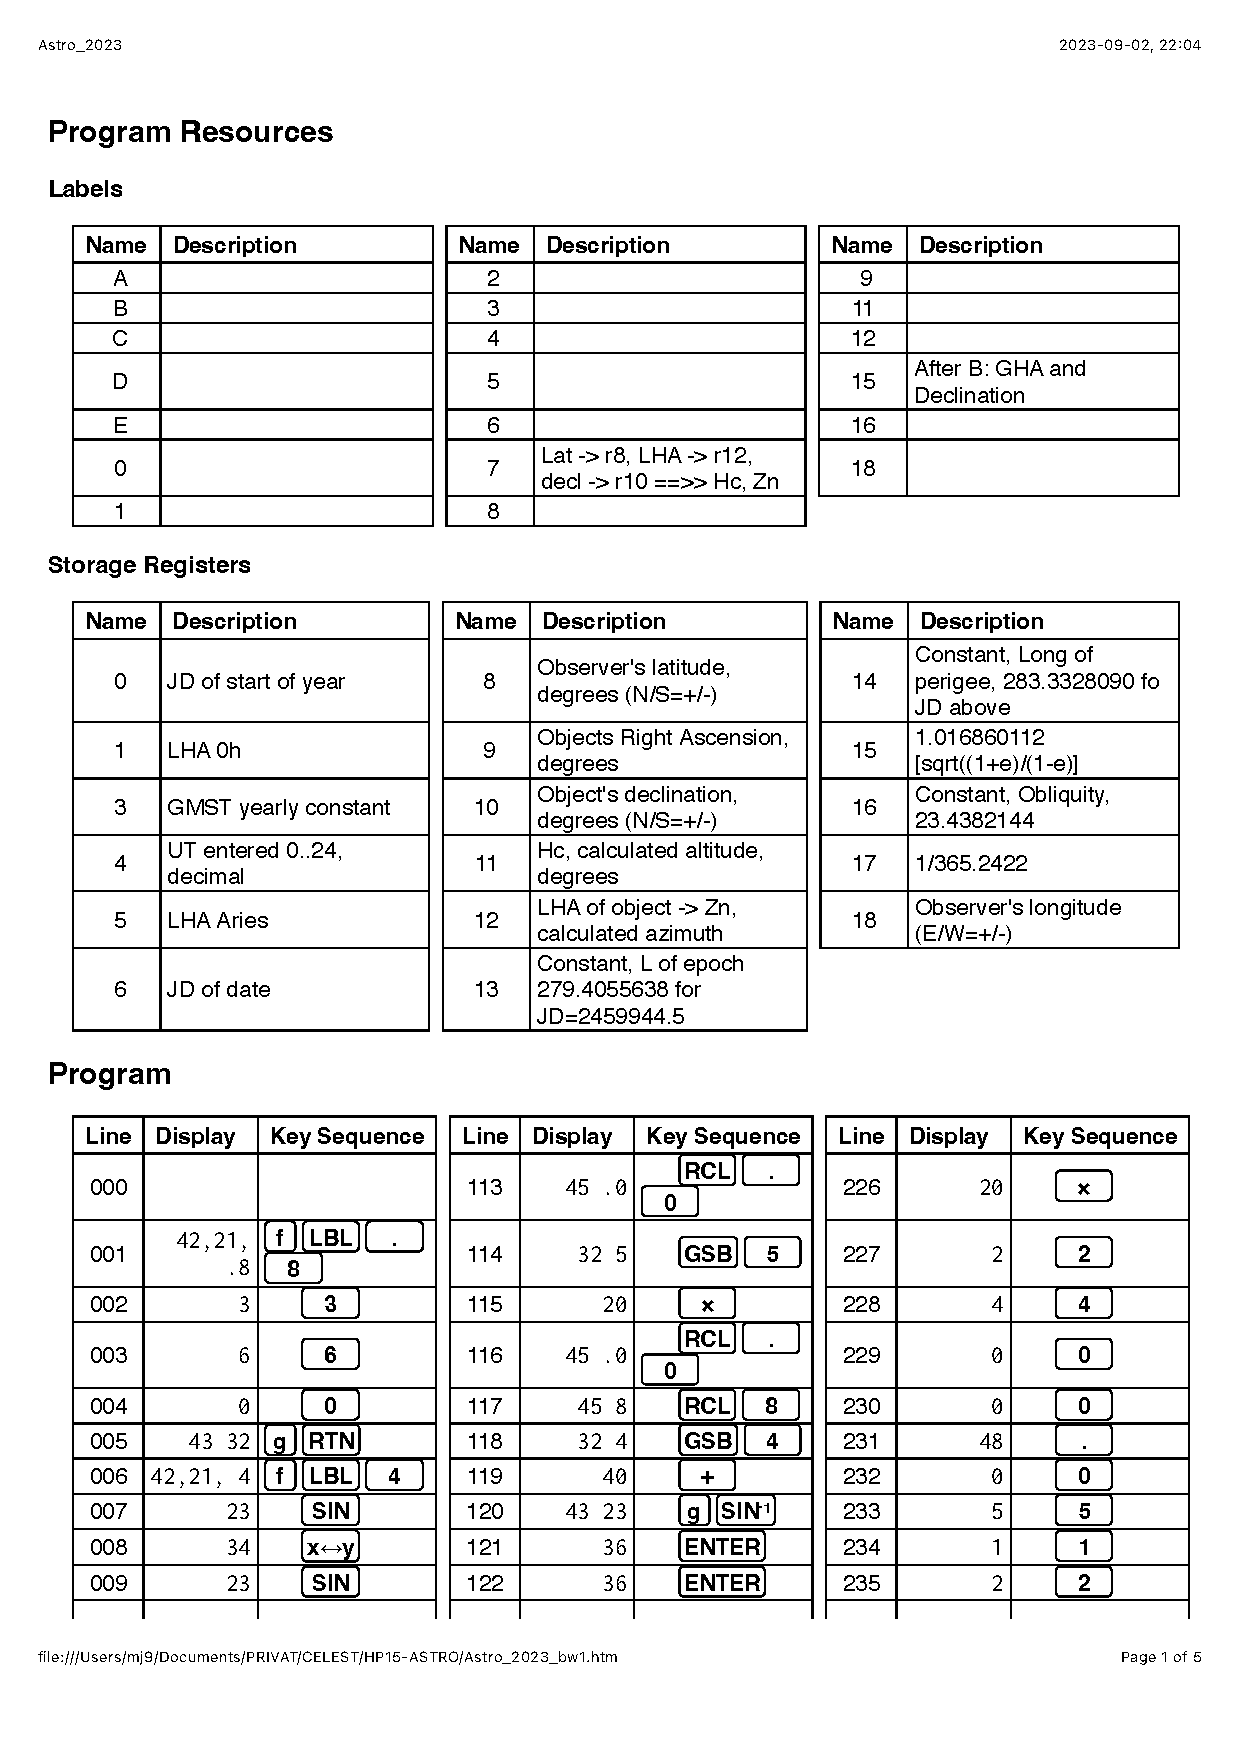
\includepdf[pages={1-5}, scale=0.9]{Astro_2023_bw.pdf}
\end{document}

